% mainfile: ../../../../master.tex
\subsection{DNA quantification with Qubit\texttrademark ~dsDNA BR Assay Kit}
% The part of the label after the colon must match the file name. Otherwise,
% conditional compilation based on task labels does NOT work.
\label{task:20180114_cj1}
\tags{dna,qnt,lab}
\authors{cj}
%\files{}
%\persons{}

According to the concentrations of DNA read by the Nanodrop, I decided to use the broad range assay kit.\sidenote{It is about 01:30 PM when I start the Qubit\texttrademark ~dsDNA BR Assay.}
\sidenote{Qubit\texttrademark dsDNA BR Assay Kit (LOT:\texttt{1835789}) was opened by Elísabet Eik Guðmundsdóttir on the \texttt{20170817}.}

First, I use 1~\uL of each of my samples for this assay, but all the values are below the detection threshold. So I repeat the assay with 5~\uL of DNA sample.

\begin{figure}[H]
    \centering
    \caption{Illustration for the Qubit\texttrademark ~DNA BR assay}
    \label{fig:20180114_dna_qnt}
    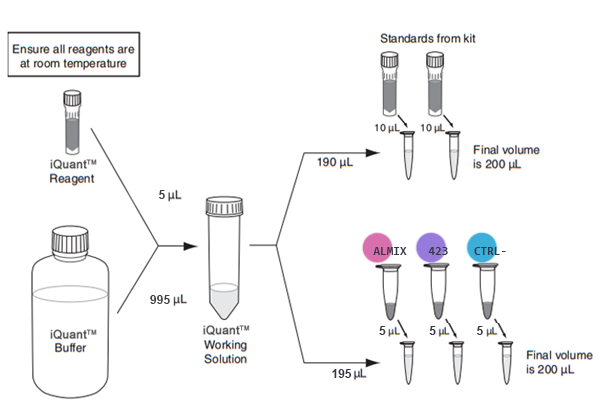
\includegraphics[width=0.7\textwidth]{graphics/schemas/20180114_dna_qnt.png}
\end{figure}

\begin{table}[H]
\caption{Total DNA quantities in samples measured with Qubit\texttrademark ~DNA BR Assay Kit}
\label{tab:20180114_nuc_acid_qnt}
\centering
\begin{tabular}{l r r r r}
\toprule
Sample ID & \textmu g/mL & $V_f$ (mL) & m (\textmu g) & m (ng) \\ \midrule\texttt{DNA\_ALMIX} & 0.776 & 0.042 & 0.032 & ~32 \\
\texttt{DNA\_423} & TOO LOW & 0.042 & NA & NA \\
\texttt{DNA\_CTRL} & TOO LOW & 0.042 & NA & NA \\
\bottomrule
\end{tabular}
\end{table}

This means I have not been able to extract the DNA from the bacterial cultures. I am starting to think that I should really reconsider this protocol, and maybe just split my samples to process separately the DNA extraction and the RNA extraction.

\comment{The weather is really bad (snow storm) so I leave at 3:20 PM to pick up Tómas in Hafnarfjörður.}